% !TEX root = ../thesis.tex

\add{Graphical models, DAGs, HC theorem}

\section{Inference on Markov Random Fields}

\add{general statement that follow presentation from W\&J + discuss general inference methods, sampling and message passing}

%%%%%%%%%%%
\subsection{\label{subsection: mrf}Markov Random Fields}

\add{rephrase section, define and use cond. indep}

%
A \margnote{MRF}\emph{Markov random field} (MRF) allows to represent specific conditional dependences between a set of random variables with a graph. 
In this report, we consider graphs determined by a finite index set $\mathcal V$, a set of edges $\mathcal E\subseteq \mathcal V\times \mathcal V$ connecting those nodes and potential functions on its cliques. Each node $i\in\mathcal V$ corresponds to one random variable taking values in a sample space $\mathcal X_i \subseteq\mathbb R^{d_i}$ for some dimension $d_i\in\mathbb N$. We restrict ourselves to graphs with pairwise interactions i.e., uniquely determined by potential functions on their nodes and edges.\add{properties, measurability} 
%Only considering pairwise MRF is not too constraining since any MRF can be reduced to a pairwise MRF by the introduction of auxiliary variables.\foot{Although this may lead to a very complex graph, see \citet{wainwright08} and references therein.} 
Consequently, we write\check{jun22}
%
\eqa{	
	\psi_i : \mathcal X_i \to \mathbb R^{+}, \quad \text{and}\quad \psi_{ij}: \mathcal X_i\times \mathcal X_j \to \mathbb R^{+}, \nn	
}
% 
respectively a potential function on a node $i\in \mathcal V$ and on an edge $(i,j)\in \mathcal E$. 
%Note that, in principle, any MRF can be 
Such a graph represents the factorisation structure of a class of probability density functions on the product space $\mathcal X := \prod\mathcal X_{i}$ that can be written as
\eqa{		p(x) &\propto & \prod_{i\in\mathcal V}\psi_{i}(x_{i})\prod_{j\in\partial i}\psi_{ij}(x_{i},x_{j}),	}
where $x=(x_{i})_{i\in \mathcal V}$ and $\partial i:=\{j\st (i,j)\!\in\,\!\mathcal E\}$ denotes the neighbourhood of the $i$th node. Note that any graphical model can be represented as a pairwise MRF \citep{yedidia00, yedidia01, wainwright08}. 
A simple pairwise MRF is illustrated in \fig{fig:simple-MRF}.\\

\begin{figure}[!h]
\center
\begin{tikzpicture}[-,>=stealth',shorten >=1pt,minimum size=0.8cm,scale=.1,node distance=1.5cm, thick]
	\node[circle,draw] (A) 						{$w$};
	\node[circle,draw] (B) [above of=A] 		{$x$};
	\node[circle,draw] (C) [below right of=A] 	{$z$};
	\node[circle,draw] (D) [below left of=A] 	{$y$};
	
	\path 
	(A) edge	(B)
	(A) edge	(C)
	(A) edge	(D)
	;
\end{tikzpicture}
\caption{\label{fig:simple-MRF}Illustration of a simple MRF corresponding to distributions over 4 random variables admitting the following factorisation structure:\\ $p(w,x,y,z)\propto \psi_{w}(w)\psi_{x}(x)\psi_{y}(y)\psi_{z}(z)\psi_{wx}(w,x)\psi_{wz}(w,z)\psi_{wy}(w,y)$.}
\end{figure}
%The node potentials usually correspond to the likelihood of some observations $y_i$ (possibly a collection of observations) such that they can be written
%\eqa{ \psi_i(x_i) &=& p_i(y_i\st x_i),	\nn	}
%for some likelihood model $p_i$.
In this work, we are mainly concerned in determining or approximating  \emph{marginals}\margnote{marginals} on the MRF i.e. the distributions $p_{\mathcal I}(x_{\mathcal I})$ for $\mathcal I\subseteq\mathcal V$  with
\eqa{		p_{\mathcal I}(x_{\mathcal I}) &:=& \int p(x_{\mathcal V\backslash \mathcal I})\dx_{\mathcal V\backslash\mathcal I}	\label{eq:marginals}.}
A particular case of interest is $\mathcal I=\{r\}$ corresponding to the case of singleton marginals.\add{Discuss why} The integrals of the form \eqref{eq:marginals} are typically intractable but exploiting the underlying factorisation structure can lead to good approximation methods.\check{jun22}

We distinguish between two classes of undirected graph structures: the connected acyclic ones (\emph{trees}) and the rest (\emph{loopy graphs}). As the rest of this document will make clear, computing marginals on a tree is relatively simple in comparison to doing so on loopy graphs. 
Among the trees, two graph structures are of particular interest in this document: the \emph{chain graph} and the \emph{star graph}. 
We also illustrate one specific type of loopy graph: the \emph{grid graph}.\check{jun22}

%\dred{COULD ADD hierarchical model as tree graph}

%%%%%%%%%%%
\subsection{Examples of MRF}
In this point, we present a brief overview of three examples of graph structures on which we will focus most of our effort throughout this document. 
We also present the type of applications they are connected with. 
They will be considered in more details in subsequent sections.\add{link to section}

%%%%%%%%%%%%%%
\subsubsection{Hidden Markov Models}
Chain graphs form the underlying structure of \emph{Hidden Markov Models} (HMM)\margnote{HMM}. These can be illustrated as follows:
\begin{figure}[!h]
\center
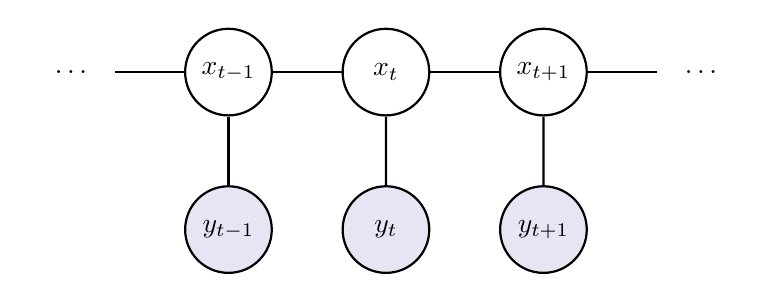
\begin{tikzpicture}[-,minimum size=1.1cm,scale=.1,node distance=2cm, thick]
	\node[circle,draw] (A) {$x_{t-1}$};
	\node[circle,draw] (B)[right of=A] {$x_{t}$};
	\node[circle,draw] (C) [right of=B] {$x_{t+1}$};
	\node[] (D) [right of=C] 	{$\dots$};
	\node[] (E) [left of=A]		{$\dots$};
	\node[circle,fill=DarkBlue!10,draw] (F) [below of=A] {$y_{t-1}$};
	\node[circle,fill=DarkBlue!10,draw] (G) [below of=B] {$y_{t}$};
	\node[circle,fill=DarkBlue!10,draw] (H) [below of=C] {$y_{t+1}$};
	
	\path 
	(A) edge	(B)
	(B) edge	(C)
	(C) edge	(D)
	(E) edge	(A)
	(A) edge (F)
	(B) edge (G)
	(C) edge (H)
	;
\end{tikzpicture}
\caption{\label{fig: hmm1} HMM with states $\{x_{t}\}_{t=1}^{T}$ and observations $\{y_{t}\}_{t=1}^{T}$.}
\end{figure}

HMMs are used in a broad range of applications from modelling time series data to speech processing \citep{ghahramani01}.\addref In HMMs, the node potentials correspond to the likelihood of the corresponding observation and the edge potentials correspond to the \emph{transition density}:\addref
\eqa{	\psi_t (x_t) &=& p(y_t\st x_t), \quad\text{and}\quad \psi_{t-1,t}(x_{t-1},x_t) \spe p(x_t\st x_{t-1}).	\nn}
A prior $\pi_{0}(x_{1})$ is assumed to be given for the first node so that $p(x_1\st y_{1}) \propto \pi_{0}(x_1)p(y_1\st x_1)$. In this case,\add{clarify which case} obtaining or approximating the singleton marginals is known as a \emph{smoothing problem}\margnote{smoothing}. The marginals or \emph{smoothing densities} can be written $p(x_t\st y_{1:T})$ to make explicit the dependence on all available observations.

A particular case is the \emph{filtering problem}\margnote{filtering} where one is only interested in building the last singleton marginal or, to put the problem in the same framework as before, to build marginals taking only into account the observations available until the point considered. The densities of interest can therefore be written $p(x_t\st y_{1:t})$.\add{discuss also smoothing problem and discuss how it's a marginal of the general thing.}\add{discuss also prediction density, discuss Chapman Kolmogorov}\check{june22}
%This is particularly relevant for applications such as time series analysis.\\

The \emph{linear-Gaussian} case is a particular instance of HMM, usually expressed as:
\eqa{	\syst{
			\pi_{0}(x_1) 				&=& \mathcal N(x_1; \mu_0, Q_0)	 	\\
			p(x_t\st x_{t-1}) 	&=& \mathcal N(x_t; A_t x_{t-1}+a_t, Q_t)		\\
			p(y_t\st x_t) 		&=& \mathcal N(y_t; B_t x_t+b_t, R_t)
		}
	\nn}
where $\mu_0$ as well as the $Q_i$, $R_i$, $A_i$, $a_i$, $B_i$ and the $b_i$ are deterministic. In such a case, an analytical expression for both the filtering and the smoothing densities can be obtained through the well-known \emph{Kalman filter} and \emph{smoother} \citep{anderson79}. 

In the general case however, where the transition is nonlinear and/or non-Gaussian, the marginals are typically intractable. Approximation algorithms such as \emph{sequential Monte Carlo} (SMC)\margnote{SMC} methods have been developed in order to generate approximate samples from these marginals and consequently be able to form Monte Carlo estimators. \addref\add{link to section} 
%We will show in this document a novel method to exploit a variational method known as \emph{expectation propagation} to help the performances of SMC smoothing algorithms. \dred{ADD SECTION NUMBER}

%%%%%%%%%%%%%%
\subsubsection{Star graphs}

In this document, we define \emph{star graphs}\margnote{star graph} as corresponding to a structure with a single random variable (possibly high-dimensional) with a node potential that factors into several likelihood terms. The structure is illustrated in the \fig{fig:star1}. 

\begin{figure}[!h]
\center
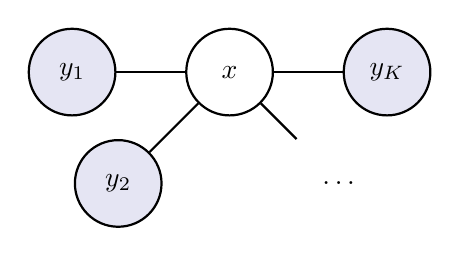
\begin{tikzpicture}[-,minimum size=1.1cm,scale=.1,node distance=2cm, thick]
	\node[circle,draw] (A) {$x$};
	\node[circle,fill=DarkBlue!10,draw] (B) [left of=A]		   {$y_{1}$};
	\node[circle,fill=DarkBlue!10,draw] (C) [below left of=A]  {$y_{2}$};
	\node[] (D) [below right of=A] {\dots};
	\node[circle,fill=DarkBlue!10,draw] (E) [right of=A]  {$y_{K}$};
	
	\path 
	(A) edge	(B)
	(A) edge	(C)
	(A) edge	(D)
	(A) edge (E)
	;
\end{tikzpicture}
\caption{\label{fig:star1} Star graph with hidden state $x$ and observations $\{y_k\}_{k=1}^{K}$. }
\end{figure} 

In this case, the singleton marginal can be written as:
\eqa{	p(x\st y) &\propto& \pi_0(x) \prod_{i=1}^{K} p(y_k\st x)	\nn}
where the $y_k$ are subsets of the entire observed data and $\pi_0$ is a prior on the hidden state. This can be a useful representation for distributed inference where each of the observation node can correspond to a distinct physical machine with a portion of the relevant data.\add{add link to section}\check{jun21}% We exploited this structure to come up with a novel way to perform distributed Bayesian inference. \dred{ADD SECTION NUMBER}

\subsubsection{Grid and loopy graphs}
The examples listed above do not exhibit cycles. An example of a common MRF structure with cycles which is encountered, for instance, in image processing, is the \emph{grid graph}\margnote{grid graph} illustrated in \fig{fig:grid1} \citep{blake11}.

\begin{figure}[!h]
	\center
	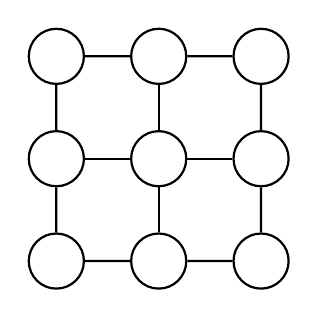
\begin{tikzpicture}[-,minimum size=.7cm,scale=.1,node distance=1.3cm, thick]
		\node[circle,draw] (A){};
		\node[circle,draw] (B) [left  of=A] {};
		\node[circle,draw] (C) [right of=A]{};
		\node[circle,draw] (D) [below of=A]{};
		\node[circle,draw] (E) [above of=A]{};
		\node[circle,draw] (F) [above of=B]{};
		\node[circle,draw] (G) [above of=C]{};
		\node[circle,draw] (H) [below of=B]{};
		\node[circle,draw] (I) [below of=C]{};
		\path
		(A) edge (B)
		(A) edge (C)
		(A) edge (D)
		(A) edge (E)
		(B) edge (F)
		(B) edge (H)
		(C) edge (I)
		(C) edge (G)
		(F) edge (E)
		(E) edge (G)
		(H) edge (D)
		(D) edge (I)
		;
	\end{tikzpicture}
\caption{\label{fig:grid1} Generic structure of a grid graph.}
\end{figure}

In image processing, grid graphs can be used to model interaction between the pixels of an image. In the case of image denoising for example, for each pixel $k$ a noisy value $y_k$ is observed and we can have a model for the likelihood of $y_k$ given the true pixel value $x_k$ in the form $p(y_k\st x_k)$. These  form the node potentials. 
Additionally, we may have a similarity measure which can be used to penalise neighbouring pixels being very dissimilar. These form the edge potentials.\\
The problem of finding or approximating the singleton marginals then corresponds to finding the likelihood of a particular pixel taking a specific value given all the noisy observations available.\check{jun21}\add{maybe link to relevant section} %\dred{ADD SECTION NUMBER WHERE WE SHOW HOW TO DO THIS}

